\documentclass[aspectratio=1610,mathserif]{beamer}
\usepackage{stmaryrd}
\usepackage{cmll}
\usepackage{tikz-cd}
\usepackage{ebproof}
\usepackage[normalem]{ulem}
\usecolortheme{rose}

\newcommand\divtok{{\circlearrowleft}}

\begin{document}

\frame\tableofcontents

\section{Introduction} %{{{
\frame\sectionpage

\begin{frame}{Context} %{{{
  State of the art:
  \begin{itemize}
    \item Verification of data structures and algorithms largely solved
    \begin{itemize}
      \item traditional program logics
    \end{itemize}
    \pause
    \item One-off verification of larger systems
    \begin{itemize}
      \item DARPA helicopter, DeepSpec, specific CPS
    \end{itemize}
    \pause
    \item Reuse of verified components is on a case-by-case basis
  \end{itemize}

  \vfill\pause
  Impact of LLMs:
  \begin{itemize}
    \item Capabilities could make verification more accessible
    \item Unreliability could be addressed by verification
  \end{itemize}
\end{frame}
%}}}

\begin{frame}{Challenge: Next-scale verification} %{{{
  How can we verify complex systems end-to-end, involving for example:
  \begin{itemize}
    \item multiple hosts communicating over a network;
    \begin{itemize}
      \item cloud application with local and remote components
    \end{itemize}
    \pause
    \item hardware devices interfacing with external world;
    \begin{itemize}
      \item NIC driver, random source, local or remote storage
    \end{itemize}
    \pause
    \item economic incentives, etc.
    \begin{itemize}
      \item economically secure blockchain protocol
    \end{itemize}
  \end{itemize}

  \vfill\pause
  This will require:
  \begin{itemize}
    \item modeling aspects of the external world compositionally;
    \item reuse of existing certified software;
    \item coarse-grained compositionality.
  \end{itemize}
\end{frame}
%}}}

\begin{frame}{Challenge: Reliable LLM agents} %{{{
  LLM-based agents act on the external world on behalf of the user. \\
  They are versatile but unreliable.

  \vfill\pause
  A well-designed verification infrastructure could address this:
  \begin{itemize}
    \item user provides a highly abstracted, declarative spec of intended action;
    \item agent generates script and proves it achieves the goal;
    \item harness validates the proof before execution.
  \end{itemize}

  \vfill\pause
  Difficulties:
  \begin{itemize}
    \item As before: external world, reuse, etc.
    \item Connecting high-level concepts (bank, USPS) to shell scripts
    \item Action-specific concepts involved, fixed model insufficient
  \end{itemize}
\end{frame}
%}}}

\begin{frame}{Research question}
  \begin{center}
    What methodologies, tools, and foundations would make this possible?
  \end{center}

  \vfill\pause
  Our conjecture:
  \begin{itemize}
    \item The ingredients already exist but must be unified
  \end{itemize}

  \vfill\pause
  They include:
  \begin{itemize}
    \item Systematic approaches to semantics
      (categorical semantics)
    \item Operational interfaces and encapsulation
      (game semantics, coalgebra)
    \item Relationship of side-effects and algebraic structures
      (algebraic effects)
    \item Connections between models
      (dualities, adjunctions)
  \end{itemize}
\end{frame}

\begin{frame}[fragile]{Proposed work}
%  We will investigate a systematic approach to heterogeneous verification:
%  \begin{itemize}
%    \item Foundations for compositional reuse of certified software
%    \item Mechanize in Rocq, connect to CompCert, ITrees, Iris
%    \item Explore applications
%  \end{itemize}
%  Our approach uses insights from
%  algebraic effects, universal coalgebra, game semantics to enable:
  We will develop mechanized foundations and frameworks for:
  \begin{itemize}
    \item Constructing semantic spaces \emph{\`a la carte} from combinations of features
    \item Characterizing semantic spaces used in existing projects
    \begin{itemize}
      \item can account for a broad range of operational and denotational approaches
      \item integrate CompCert, ITrees, Iris
    \end{itemize}
    \item Transporting specs, semantics and proofs across those spaces.
    \item Coarse-grained composition of systems, state, abstraction layers.
  \end{itemize}
\end{frame}

\begin{frame}{Application: Shell commands}
  We will demonstrate our framework with the running example:
  \begin{align*}
    c \in \mathbf{cmd} ::= {} &
      \texttt{true} \mid
      \texttt{false} \mid
      \texttt{!}c \mid
      c_1 \mathbin{\texttt;} c_2 \mid
      c_1 \mathbin{\texttt{\&\&}} c_2 \mid
      c_1 \mathbin{\texttt{||}} c_2 \mid {}
      & \text{(pure)}
      \\&
      \texttt{echo} \, s \mid
      \texttt{tail -}n \mid
      c \:\: n_1 \mathbin{\texttt{>\&}} n_2 \mid {}
      & \text{(I/O effects)}
      \\&
      \texttt{yes} \mid
      \texttt{sort} \mid
      \texttt{uniq} \mid
      \texttt{while } c_1 \texttt{ do } c_2 \mid {}
      & \text{(non-termination)}
      \\&
      \texttt{shuf} \mid {}
      & \hspace{-4em} \text{(non-determinism, probability)}
      \\&
      c_1 \mathbin{\texttt{\&}} c_2 \mid
      c_1 \mathbin{\texttt{|}} c_2 \mid {}
      & \text{(concurrency)}
      \\&
      \mathsf{load}(\texttt{foo.s})
      & \text{(user program)}
  \end{align*}
\end{frame}

\frame{}

\begin{frame}{Semantics} %{{{
  The story goes:
  \begin{itemize}
    \item \textbf{Syntax:}
      a type of ``blueprints'' for describing the systems we wish to study \\
      (program text, circuit diagram, floor plans)
    \pause
    \item \textbf{Semantic model:}
      \begin{itemize}
        \item a mathematical semantic \textbf{space} (domains, ODEs, etc) \\
          where we can carry out formal reasoning, together with
        \item a semantic \textbf{interpretation} of the syntactic objects \\
          into this space (denotation function, rules for circuits, etc).
      \end{itemize}
  \end{itemize}

  \vspace{1em}
  \[
    \text{Abstract Syntax} \:
    \xrightarrow[\llbracket - \rrbracket]{\text{Semantic Interpretation}} \:
    \text{Semantic Space}
  \]
\end{frame}
%}}}

\begin{frame}{Compositionality} %{{{
  To verify complex systems, we need to isolate components:
  \begin{itemize}
    \item The \emph{interface} of a component
      carefully limits the ways in which it can interact
      with the rest of the system.
    \item Its internal state is encapsulated
      and we can assume noninterference to reason about
      the behavior of each component.
  \end{itemize}

  \pause \vspace{1em}
  We will often focus on various kinds of \emph{objects}:
  \begin{itemize}
    \item a signature spells out the methods which clients can invoke;
    \item the object updates its state in response to
      each methods invocation.
  \end{itemize}

  \pause \vspace{1em}
  However, we want to support \emph{heterogeneous} systems
  made up of parts with various interfaces,
  and reason across a range of abstraction levels.
\end{frame}
%}}}

\begin{frame}{Heterogeneous Verification} %{{{
  \textbf{Vision} outlined in the POPL 2025 paper:
  \[
    \includegraphics[scale=0.27]{sem}
  \]

  \pause
  \textbf{Challenge:} reusing and interfacing semantic models
    from various projects

  \pause
  \vspace{1em}
  \textbf{Proposal:}
  uniform framework for characterizing existing semantic spaces, \\
  constructing new ones, defining embeddings back and forth.
\end{frame}
%}}}

\begin{frame}<0>{Terminology} %{{{
  Important to distinguish:
  \begin{itemize}
    \item Semantic space: set with extra structure (algebra, coalgebra, dcpo)
    \item Semantic model: space + interpretation of some language
    \item Semantic paradigm: denotational sem, operational, game semantics
    \item Semantic framework (ITrees, CCR, CompCertO)
  \end{itemize}
\end{frame}
%}}}

\begin{frame}<0>{Big picture} %{{{
We are proposing a semantic framework
for heterogeneous verification.
\begin{itemize}
  \item Characterize various semantic spaces in a uniform framework
  \item Define embeddings, etc
  \item Methodology for defining new ones from combination of features
\end{itemize}

\vspace{1em}
Building blocks will allow us to handle and combine
\begin{itemize}
  \item Interaction trees
  \item Choice trees
  \item CompCert/CompCertO semantics
  \item Certified abstraction layers
\end{itemize}
\end{frame}
%}}}

\begin{frame}{Complicating the story} %{{{
  In reality things are not so clear-cut:
  \begin{itemize}
    \item Are these syntax or semantics?
      \begin{itemize}
        \item $\lambda$-terms under $\beta$-reduction
        \item circuit diagrams
        \item interaction trees
        \item \ldots
      \end{itemize}
    \pause
    \item Abstract syntax is already
      a formal mathematical object
    \pause
    \item If we build a heterogeneous model
      by assembling semantic objects, \\
      is that syntax or semantics?
  \end{itemize}

  \pause
  \vspace{1em}
  So in general, more like
  \[
    \text{Mathematical setting A} \:
    \xrightarrow[\llbracket - \rrbracket]{\text{Interpretation}} \:
    \text{Mathematical setting B}
  \]
\end{frame}
%}}}

\begin{frame}{What do we want from a semantic model?} %{{{
  \begin{itemize}
    \item Make the operational behavior of the system explicit.
      \begin{itemize}
        \item Use a standardized, already-understood semantic space \\
          (input--output functions, free monad, interaction trees).
        \item Define a \textbf{coalgebra} on the semantic space
           to tell you ``what happens next''.
      \end{itemize}
      This is the aspect most favored by \textbf{operational} semantics.
    \pause
    \vspace{1ex}
    \item Make it easy to build new semantic objects from their constitutents.
      \begin{itemize}
        \item Work within an \textbf{ambient category} of well-known algebraic structures \\
          (domains for recursion,
           semilattices for nondeterminism, etc).
        \item Provide additional operations that make sense in the context
          (an \textbf{algebra}).
      \end{itemize}
      This helps with defining a \textbf{denotational} interpretation.
  \end{itemize}
\end{frame}
%}}}

%}}}

\section{Alt.\@ Intro} %{{{
\frame\sectionpage

\begin{frame}{Challenges for End-to-End Verification}
  \begin{itemize}
    \item Scale requires compositionality and reuse
    \item Interfacing certified components of different natures
    \item Working across abstraction levels and granularities
    \item Theoretical support and tools underdeveloped
  \end{itemize}
\end{frame}

\begin{frame}{Interfaces}
  To control complexity and scale, we must use encapsulated components:
  \begin{itemize}
    \item Internal state hidden from the rest of the system
    \item Interactions happen across a well-defined interface
    \item External behavior of components is what matters
  \end{itemize}

  \vspace{1ex}
  Examples:
  \begin{itemize}
    \item Input--output functions $\llbracket \Gamma \vdash M : \tau \rrbracket$
    \item Objects accessed through a fixed set of methods
    \item Free monad for uninterpreted external effects
  \end{itemize}
\end{frame}

\begin{frame}{Games as interface}
  \emph{Games} are a versatile way to describe the interfaces of components:
  \begin{itemize}
    \item Subsume input--output, object interfaces, effect signatures
    \item Can incorporate a sequential dimension and vary across time
  \end{itemize}
  The behavior of components is described by \emph{strategies}.

  \vspace{1em}
  Game semantics uses this approach successfully
  to reconcile \\ denotational semantics and
  sequentiality-sensitive features.
\end{frame}

\begin{frame}
  Strategy models have been defined that deal with
  \begin{itemize}
    \item Non-termination
    \item State
    \item High-order types
    \item Nondeterminism
    \item Probabilistic behavior
    \item Concurrency
    \item \ldots
    \item and combinations thereof
  \end{itemize}

  \vspace{1em}
  However, existing approaches are ad-hoc:
  \begin{itemize}
    \item Propose a model for a combination of features
    \item Show that it exhibits the required structure and properties
  \end{itemize}
\end{frame}

\begin{frame}{Our approach}
  Decouple structure of the game from strategy construction
  \begin{enumerate}
    \item Complex games can be ``compiled'' down
      to simple alternating games
    \item Use systematic approach to defined strategy spaces
      for those simple games
  \end{enumerate}

  \vspace{1ex}
  Under this approach:
  \begin{itemize}
    \item Features affecting the combinatorial shape of games
      reflected in \#1
    \item Features related to ambient effects
      reflected in \#2.
  \end{itemize}

  \vspace{1ex}
  We do this by reusing theory and techniques from algebraic effects, \\
  and call the resulting framework algebraic game semantics.
\end{frame}
%}}}

\section{Basic Approach} %{{{
\frame\sectionpage

\begin{frame}[fragile]{Algebraic Game Semantics} %{{{
  Game semantics uses \emph{games} as
  an intermediate description of semantic spaces
  \[
    \begin{tikzcd}[sep=8em]
      \text{Game}
      \ar[r, mapsto, "\text{Strategy space}"] &
      \text{Domain}
    \end{tikzcd}
  \]
  however the ``strategy space'' constructions are ad-hoc.

  \pause
  \vspace{1em}
  We borrow concepts and techniques from
  \begin{itemize}
    \item Algebraic effects
    \item Universal Coalgebra
  \end{itemize}
  to provide a new foundation for game semantics.
\end{frame}
%}}}

\begin{frame}{Example: the Monty Hall problem} %{{{
  The \emph{Monty Hall problem} involves a game
  with a prize hidden behind one of 3 doors:
  \begin{enumerate}
    \item the participant ``$\Sigma$'' chooses one of the doors;
    \item the host ``$\Pi$'' opens another, loosing door;
  \[
    \includegraphics{Monty_open_door}
  \]
    \item the participant may switch their choice to the remaining door.
  \end{enumerate}
  Then the host opens the chosen door to reveal whether the prize is won.

  \pause
  \vspace{1em}
  The original problem asks whether switching at step 3 gives us an advantage. \\
  However for now we will only focus on the interaction itself.
\end{frame}
%}}}

\begin{frame}[fragile]{Example: Monty Hall strategy space} %{{{
  The Monty Hall interaction, and one of the strategies, can be depicted as:
  \[
    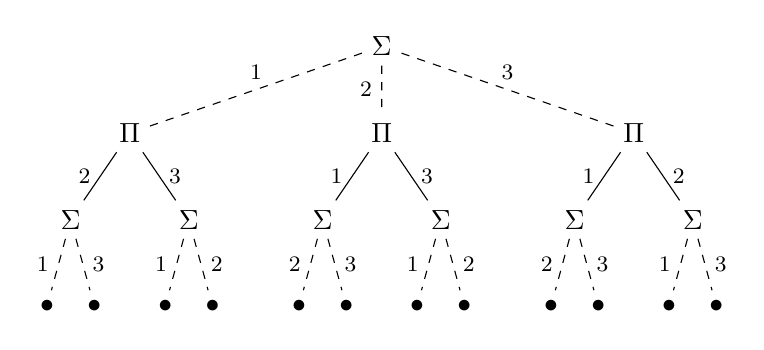
\begin{tikzpicture}
      [baseline=(B.base),
       level distance=11mm,
       level 1/.style={sibling distance=3.2cm,edge from parent/.style={draw,dashed}},
       level 2/.style={sibling distance=1.5cm,edge from parent/.style={draw,solid}},
       level 3/.style={sibling distance=0.6cm,edge from parent/.style={draw,dashed}},
       every node/.style={font=\footnotesize},
       every child node/.style={font=\normalsize}]
      \node[font=\normalsize] {$\Sigma$}
        child {
          node {$\Pi$}
          child {
            node {$\Sigma$}
            child { node {$\bullet$} edge from parent node[left] {$1$} }
            child { node {$\bullet$} edge from parent node[right] {$3$} }
            edge from parent node[left] (B) {$2$}
          }
          child {
            node {$\Sigma$}
            child { node {$\bullet$} edge from parent node[left] {$1$} }
            child { node {$\bullet$} edge from parent node[right] {$2$} }
            edge from parent node[right] {$3$}
          }
          edge from parent node[above] {$1$}
        }
        child {
          node {$\Pi$}
          child {
            node {$\Sigma$}
            child { node {$\bullet$} edge from parent node[left] {$2$} }
            child { node {$\bullet$} edge from parent node[right] {$3$} }
            edge from parent node[left] {$1$}
          }
          child {
            node {$\Sigma$}
            child { node {$\bullet$} edge from parent node[left] {$1$} }
            child { node {$\bullet$} edge from parent node[right] {$2$} }
            edge from parent node[right] {$3$}
          }
          edge from parent node[left] {$2$}
        }
        child {
          node {$\Pi$}
          child {
            node {$\Sigma$}
            child { node {$\bullet$} edge from parent node[left] {$2$} }
            child { node {$\bullet$} edge from parent node[right] {$3$} }
            edge from parent node[left] {$1$}
          }
          child {
            node {$\Sigma$}
            child { node {$\bullet$} edge from parent node[left] {$1$} }
            child { node {$\bullet$} edge from parent node[right] {$3$} }
            edge from parent node[right] {$2$}
          }
          edge from parent node[above] {$3$}
        }
        ;
    \end{tikzpicture}
    \qquad
    \qquad
    \begin{tikzpicture}
      [baseline=(B.base),
       level distance=11mm,
       %every child node/.style={draw,circle},
      ]
      \node {$\uline2$} child {
        node {$\langle \rangle$}
        child {
          node {$\uline3$}
          child { node {$\langle \rangle$} edge from parent [dashed] }
          edge from parent [solid] node[left] (B) {\footnotesize $1$}
        }
        child {
          node {$\uline1$}
          child { node {$\langle \rangle$} edge from parent [dashed] }
          edge from parent [solid] node[right] {\footnotesize $3$}
        }
        edge from parent [dashed]
      };
    \end{tikzpicture}
  \]
  Moreover the set of strategies for this game can be written as:
  \[
    \sum_{i \in \mathbf{3}} \:
    \prod_{j \in \mathbf{3} \setminus \{ i \}}
    \sum_{k \in \mathbf{3} \setminus \{ j \}}
    %\prod_{r \in \{\text{w}, \text{l}\}}
    \mathbf{1}
    \qquad \ni \qquad
    \only<1>{
      \iota_2 \bigl( \langle \iota_3(*), \iota_1(*) \rangle \bigr)
    }
    \only<2>{
      \uline{2} \bigl\langle \,
        \uline{3} \langle \rangle, \,
        \uline{1} \langle \rangle \,
      \bigr\rangle
    }
  \]
\end{frame}
%}}}

\begin{frame}{Strategy spaces} %{{{
  The Monty Hall example illustrates that:
  \begin{itemize}
    \item A strategy in $\sum_{i\in I} S_i \ni \iota_j(\sigma)$
      first performs a proponent choice $j \in I$, \\
      then continues with the strategy $\sigma \in S_j$.
    \item A strategy in $\prod_{i \in I} S_i \ni \langle \sigma_i \rangle_{i \in I}$
      responds to an environment choices $i \in I$ \\
      by continuing with the strategy $\sigma_i \in S_i$.
  \end{itemize}
  \pause
  \vspace{1ex}
  More generally,
  \begin{itemize}
    \item Operations on sets like $\sum X$, $\prod X$
      reflect an initial portion of the game,
      transforming a set $X$ of ``continuation'' strategies.
    \item By composing successive operations
      we can spell out \\ the sequential progression
      of the interaction.
  \end{itemize}
  Based on this idea we will use \emph{functors}
  to represent strategy space constructions for
  (sequential portions of) games
  and their (sequential) composition.
\end{frame}
%}}}

\begin{frame}[fragile]{Functors} %{{{
  \begin{definition}[Functor on sets]
    A \emph{functor} $F : \mathbf{Set} \rightarrow \mathbf{Set}$
    is a unary operation on sets
    with a transformation:
    \[
      \begin{prooftree}
        \hypo{f : X \rightarrow Y}
        \infer1{F f : FX \rightarrow FY}
      \end{prooftree}
      \quad \text{such that} \quad
      \begin{array}{c}
        F \, \mathsf{id} = \mathsf{id} \: \\
        F (g \circ f) = Fg \circ Ff
      \end{array}
    \]
  \end{definition}
  \pause
  In the context of strategy spaces we can think of $F$
  as an initial shape for a game:
  \[
    FX := X + (X \times X)
    \qquad \qquad
    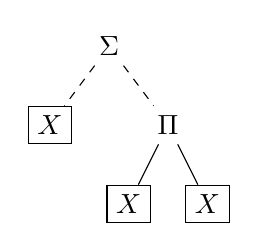
\begin{tikzpicture}
      [baseline=(B.base),
       level distance=1cm,
       level 1/.style={sibling distance=1.5cm,edge from parent/.style={draw,dashed}},
       level 2/.style={sibling distance=1cm,edge from parent/.style={draw,solid}}]
      \node {$\Sigma$}
        child { node[draw] (B) {$X$} }
        child {
          node {$\Pi$}
          child { node[draw,solid] {$X$} }
          child { node[draw,solid] {$X$} }
        };
    \end{tikzpicture}
    \quad
    \xrightarrow{\quad F f \quad}
    \quad
    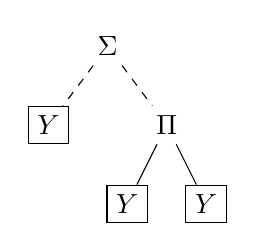
\begin{tikzpicture}
      [baseline=(B.base),
       level distance=1cm,
       level 1/.style={sibling distance=1.5cm,edge from parent/.style={draw,dashed}},
       level 2/.style={sibling distance=1cm,edge from parent/.style={draw,solid}}]
      \node {$\Sigma$}
        child { node[draw] (B) {$Y$} }
        child {
          node {$\Pi$}
          child { node[draw,solid] {$Y$} }
          child { node[draw,solid] {$Y$} }
        };
    \end{tikzpicture}
  \]
\end{frame}
%}}}

\begin{frame}[fragile]{Natural Transformations} %{{{
  \begin{definition}[Natural transformation]
    A \emph{natural} transformation
    $\phi : \forall X \cdot F X \rightarrow G X$
    is a family of functions \\ such that
    for all $f : X \rightarrow Y$,
    \vspace{-1.5em}
    \[
      \qquad \qquad
      \phi_Y \circ F f = G f \circ \phi_X
      \qquad \qquad
      \begin{tikzcd}
        F X \ar[r, "\phi X"]
            \ar[d, "F f"] &
        G X \ar[d, "G f"] \\
        F Y \ar[r, "\phi Y"] &
        G Y
      \end{tikzcd}
    \]
    \vspace{-1em}
  \end{definition}
  \pause
  $F f$ transformed the \emph{continuation} part, and
  $\phi X$ transforms the \emph{initial} portion in $FX$:
      \[ \phi : \forall X \cdot X + (X \times X) \rightarrow
                            (X + X) \times (X + X) \]
  \[
    \begin{array}{r}
      \phi_X( \iota_1(x) ) = \langle \iota_1(x), \iota_1(x) \rangle \\
      \phi_X( \iota_2(\langle x, x' \rangle) ) =
        \langle \iota_2(x), \iota_2(x') \rangle
    \end{array}
    \qquad
    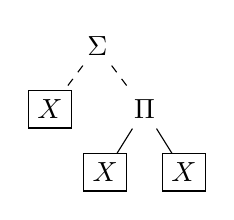
\begin{tikzpicture}
      [baseline=(B.base),
       level distance=8mm,
       level 1/.style={sibling distance=1.2cm,edge from parent/.style={draw,dashed}},
       level 2/.style={sibling distance=1cm,edge from parent/.style={draw,solid}}]
      \node {$\Sigma$}
        child { node[draw] (B) {$X$} }
        child {
          node {$\Pi$}
          child { node[draw,solid] {$X$} }
          child { node[draw,solid] {$X$} }
        };
    \end{tikzpicture}
    \:
    \xrightarrow{\: \phi X \:}
    \:
    \begin{tikzpicture}
      [baseline=(B.base),
       level distance=8mm,
       level 1/.style={sibling distance=2cm,edge from parent/.style={draw,solid}},
       level 2/.style={sibling distance=1cm,edge from parent/.style={draw,dashed}}]
      \node {$\Pi$}
        child {
          node {$\Sigma$}
          child { node[draw,solid] {$X$} }
          child { node[draw,solid] {$X$} }
        }
        child {
          node {$\Sigma$}
          child { node[draw,solid] {$X$} }
          child { node[draw,solid] {$X$} }
        };
    \end{tikzpicture}
  \]
\end{frame}
%}}}

\begin{frame}{Monty Hall functor} %{{{
  With this in mind,
  the Monty Hall protocol can be made into a functor:
  \[
    H X := 
    \sum_{i \in \mathbf{3}} \:
    \prod_{j \in \mathbf{3} \setminus \{ i \}}
    \sum_{k \in \mathbf{3} \setminus \{ j \}}
    \prod_{r \in \{\text{w}, \text{l}\}}
    X
  \]
  Note that the original strategy space can be recovered as $H \mathbf{1}$.

  \pause
  \vspace{1em}
  Monty Hall strategies define natural transformations
  $
    \sigma , \tau: \forall X \cdot X \rightarrow HX
  $ \\
  and we can construct composites like
  \[
    \sigma \tau \sigma \mathbf{1} \in HHH\mathbf{1}
  \] 

  \pause
  This view of functors as sequential components
  for building strategy spaces \\
  will form the core of our uniform approach to game semantics.
\end{frame}
%}}}

%}}}

\section{Coalgebras} %{{{
\frame\sectionpage

\begin{frame}{Definition} %{{{
  \begin{definition}[$F$-Coalgebra]
    A \emph{coalgebra} for $F : \mathbf{Set} \rightarrow \mathbf{Set}$
    is a set $S$ together with a function $\delta : S \rightarrow FS$.
  \end{definition}
  Coalgebras generalize various kinds of \emph{transition systems}.

  \pause\vfill
  Consider the set $\mathbf{2} = \{0, 1\}$
  together with a function $\delta : \mathbf{2} \rightarrow H\mathbf{2}$
  defined by:
  \begin{align*}
    \delta(0) &= \sigma 1 \\
    \delta(1) &= \tau 0
  \end{align*} 
  The states $b \in \mathbf{2}$ define strategies
  for an \emph{iterated} version of Monty Hall. \\
  The elementary strategies $\sigma$ and $\tau$ are played in alternation. \\
  The behavior represented by $0$ starts with $\sigma$,
  while $1$ starts with $\tau$.
\end{frame}
%}}}

\begin{frame}[fragile]{Homomorphisms} %{{{
  \begin{definition}[Coalgebra homomorphism]
  A coalgebra homomorphism is a map that preserves behaviors:
  \[
    \begin{tikzcd}
       (A, \alpha) \ar[d, "f"'] \\ (B, \beta)
    \end{tikzcd}
    \quad := \qquad
    \begin{tikzcd}
       A \ar[r, "\alpha"] \ar[d, "f"'] &
       FA \ar[d, "Ff"] \\
       B \ar[r, "\beta"] &
       FB
    \end{tikzcd}
    \qquad
    \beta \circ f = F f \circ \alpha
  \]
  \end{definition}

  \pause
  \vspace{1em}
  Note that $B$ is a richer or ``more complete'' space: \\
  every behavior represented in $A$ can be represented in $B$, \\
  but $B$ may contain behaviors that cannot be represented in $A$.
\end{frame}
%}}}

\begin{frame}{Terminal Coalgebra} %{{{
  In fact, there is often a ``most complete'' coalgebra:
  the \emph{terminal $F$-coalgebra}, \\
  into which there is a unique homomorphism
  for each coalgebra for the functor $F$.

  \pause
  \vspace{1em}
  Examples:
  \begin{itemize}
    \item Coinductive types
    \item Sets of traces for LTS
    \item Game semantics strategy constructions
  \end{itemize}
\end{frame}
%}}}

%}}}

\section{Algebras}
\frame\sectionpage

\section{Ambient Effects}
\frame\sectionpage

\section{Adjunctions} %{{{
\frame\sectionpage

\begin{frame}[fragile]{Interpretation}
  An adjunction $F \dashv G : \mathbf{D} \rightarrow \mathbf{C}$
  is a relationship between functors:
  \[
    \begin{tikzcd}
      \mathbf{C} \ar[rr, bend left, "F"] &
      \bot &
      \mathbf{D} \ar[ll, bend left, "G"]
    \end{tikzcd}
  \]

  Often,
  \begin{itemize}
    \item $\mathbf{D}$ is a category of spaces with more sophisticated structure
    \item $\mathbf{C}$ is a category of simpler ``underlying'' spaces
    \item $F X \in \mathbf{D}$ is the free structure generated by $\mathbf{X}$
    \item $G Y \in \mathbf{C}$ is the underlying space used in $Y$
  \end{itemize}
\end{frame}

\begin{frame}[fragile]{Example: Powerset adjunction}
  \[
    \begin{tikzcd}
      \mathbf{Set} \ar[rr, bend left, "\mathcal{P}"] &
      \bot &
      \mathbf{Sup} \ar[ll, bend left, "U"]
    \end{tikzcd}
  \]

  Here,
  \begin{itemize}
    \item $\mathcal{P} X \in \mathbf{Sup}$ is
      the free sup-lattice generated by $X \in \mathbf{Set}$
    \item $U Y \in \mathbf{Set}$ is the underlying set of
      the sup-lattice $Y \in \mathbf{Sup}$
    \item the unit $\eta_X : X \rightarrow U\mathcal{P} X \in \mathbf{Set}$
      embeds the generators into the free lattice
    \item the counit
      $\varepsilon_Y : \mathcal{P} U Y \rightarrow Y \in \mathbf{Sup}$
      evaluates $\mathbf{y} \in \mathcal{P}UY$ using
      the joins in $Y$ 
  \end{itemize}
\end{frame}

\begin{frame}[fragile]{Definition}
  \[
    \begin{tikzcd}
      \mathbf{C} \ar[rr, bend left, "F"] &
      \bot &
      \mathbf{D} \ar[ll, bend left, "G"]
    \end{tikzcd}
  \]

  \vfill
  An adjunction $F \dashv G : \mathbf{D} \rightarrow \mathbf{C}$
  is defined by an equivalence
  \[
    \phi : \forall X Y \cdot \mathbf{D}(F X, Y) \cong \mathbf{C}(X, GY)
    \quad \text{such that} \quad
    \begin{array}{c}
      \phi(f \circ u) = \phi(f) \circ F u \\
      \phi(v \circ f) = G v \circ \phi(f)
    \end{array}
  \]
  The unit $\eta : \forall X \cdot X \rightarrow GFX \in \mathbf{C}$
  and counit $\varepsilon : \forall Y \cdot FGY \rightarrow Y$
  are obtained as:
  \[
    \eta_X := \phi_{X,FX}(\mathsf{id}_{FX})
    \qquad
    \varepsilon_Y := \phi^{-1}_{GY, Y}(\mathsf{id}_{GY})
  \]
\end{frame}

\begin{frame}[fragile]{Properties}
  \[
    \begin{tikzcd}
      \mathbf{C} \ar[rr, bend left, "F"] &
      \bot &
      \mathbf{D} \ar[ll, bend left, "G"]
    \end{tikzcd}
  \]

  \vfill
  $F$ preserve coproducts and initial algebras
  \[
    F (A + B) \cong FA \oplus FB
    \qquad
    \begin{prooftree}
      \hypo{S : \mathbf{C} \rightarrow \mathbf{C}}
      \hypo{FS \cong TF}
      \hypo{T : \mathbf{D} \rightarrow \mathbf{D}}
      \infer3{F \mu S \cong \mu T}
    \end{prooftree}
  \]
  $G$ preserve products and final coalgebras
  \[
    GA \times GB \cong G (A \with B)
    \qquad
    \begin{prooftree}
      \hypo{S : \mathbf{C} \rightarrow \mathbf{C}}
      \hypo{SG \cong GT}
      \hypo{T : \mathbf{D} \rightarrow \mathbf{D}}
      \infer3{\nu S \cong G \nu T}
    \end{prooftree}
  \]
\end{frame}

\begin{frame}[fragile]{Monads From Adjunctions}
  \[
    \begin{tikzcd}
      \mathbf{C} \ar[rr, bend left, "F"] &
      \bot &
      \mathbf{D} \ar[ll, bend left, "G"]
    \end{tikzcd}
  \]

  \vfill
  Every adjunction induces a monad $GF : \mathbf{C} \rightarrow \mathbf{C}$
  and a comonad $FG : \mathbf{D} \rightarrow \mathbf{D}$
  \[
    \mu := G \varepsilon F : GFGF \rightarrow GF
    \qquad
    \bar{\mu} := F \eta G : FG \rightarrow FGFG
  \]
\end{frame}

\begin{frame}{Adjunctions From Monads}
  Given a monad $M : \mathbf{C} \rightarrow \mathbf{C}$
  there are several ways to generate a category $\mathbf{D}$
  and two functors $F \dashv G : \mathbf{D} \rightarrow \mathbf{C}$
  such that $M \cong GF$:
  \begin{itemize}
    \item the Kleisli category which has morphisms
      $\mathbf{D}(A, B) := \mathbf{C}(M A, B)$ 
    \item the Eilenberg-Moore category of \emph{monad algebras} for $M$.
  \end{itemize}

  Coproducts in $\mathbf{C}$ carry over to the Kleisli category.

  Products in $\mathbf{C}$ carry over to the EM category.

  The latter often has more structure as well.
\end{frame}

\begin{frame}[fragile]{Monad Algebras}
  A monad algebra is an object $A \in \mathbf{C}$ with a morphism
  $\alpha : MA \rightarrow A$ such that:
  \[
    \begin{tikzcd}
      A \ar[r, "\eta"] \ar[rd, =] &
      MA \ar[d, "\alpha"] \\
      & A
    \end{tikzcd}
    \qquad
    \begin{tikzcd}
      MMA \ar[r, "\mu"] \ar[d, "\alpha"] &
      MA \ar[d, "\alpha"] \\
      MA \ar[r, "\alpha"] &
      A
    \end{tikzcd}
  \]
\end{frame}

%}}}

\section{Probabilistic computations (w/ Chris)} %{{{
\frame\sectionpage

\begin{frame}{Probability monad}
  A finitely supported distribution $\delta \in \mathsf{Dist}(X)$
  over a set $X$ is an assignment
  \[ \delta : X \rightarrow [0,1] \]
  such that
  \begin{itemize}
    \item $\delta(x) = 0$ for all but a finite number of $x$s, and
    \item $\sum_{x\in X} \delta(x) = 1$.
  \end{itemize}

  \vspace{1em}
  $\mathsf{Dist}$ is a monad where $\eta(x)$
  assigns probability $1$ to $x$, \\ and $\mu$
  mixes the probabilities from a distribution of distributions.
\end{frame}

\begin{frame}{Convex spaces}
  The space $\mathsf{Dist}(X)$ is an example of a \emph{convex space},
  which is a set $D$ equipped with a \emph{convex combination} operation:
  \[
    \alpha_1 x_1 + \cdots + \alpha_n x_n
    \qquad
    \Bigl( \sum_i \alpha_i = 1 \Bigr)
  \]
  In fact, $\mathsf{Dist}(X)$ is the \emph{free convex space}
  generated by $X$.

  \vspace{1em}
  Note that $\mathbb{R}$ and every set with a notion of
  ``weighted average'' are convex spaces.
\end{frame}

\begin{frame}[fragile]{Adjunction}
  More precisely, there is an adjunction
  $\mathsf{Dist} \dashv U : \mathbf{Conv} \rightarrow \mathbf{Set}$:
  \[
    \begin{tikzcd}
      \mathbf{Set} \ar[rr, bend left, "\mathsf{Dist}"] &
      \bot &
      \mathbf{Conv} \ar[ll, bend left, "U"]
    \end{tikzcd}
  \]
  The category $\mathbf{Conv}$ is:
  \begin{itemize}
    \item Complete (giving us $\with, \nu$)
    \item Cocomplete ($\oplus, \mu$)
    \item Symmetric monoidal closed ($\otimes$, $\multimap$)
  \end{itemize}
\end{frame}

\begin{frame}{Expectation values}
  The universal property of the adjunction gives us a way
  to compute expectation values.

  For example, consider the payoff function
  $p : \{W,L\} \rightarrow U\mathbb{R}$
  defined by
  \[ p(W) = \$90 \qquad p(L) = \$0 \]
  Its transpose $p^\dagger : \mathsf{Dist}(X) \rightarrow \mathbb{R}$
  is
  \[ p^\dagger(\alpha \cdot W + \beta \cdot L) =
     \alpha \cdot \$90 + \beta \cdot \$0 \]
  For example:
  \[ p^\dagger \Bigl( \frac{1}{3} W + \frac{2}{3} L \Bigr) =
      \$30 \]
\end{frame}

%\begin{frame}{Example: Monty Hall strategies}
%\small
%\begin{verbatim}
%Monty Hall "server":
%w <- uniform(3) ;
%i : 3 .
%j <- uniform(3 \ {i}) ; iota_j (
%k : 3 \ {j} . eta(W) if k = w
%              eta(L) otherwise
%\end{verbatim}
%\end{frame}

%}}}

\section{Information flow control (w/ Chris)} %{{{
\frame\sectionpage

\begin{frame}{Views}
  If we have a principal lattice $L$,
  we can provide ``views'' for each principal,
  each taken in a set $(X_\ell)_{\ell \in L}$,
  such that for all $\ell_1 \le \ell_2$
  we have a projection
  \[ f : X_{\ell_2} \rightarrow X_{\ell_1}  \,. \]
  The projections should be consistent with one another.

  \vspace{1em}
  The category $[L^\mathrm{op}, \mathbf{Set}]$ has:
  \begin{itemize}
    \item Tuples $(X_\ell)_{\ell \in L}$ and associated projections
      as objects
    \item Functions $(f_\ell : X_\ell \rightarrow Y_\ell)$
      which commute with the projections as morphisms
  \end{itemize}
\end{frame}

\begin{frame}[fragile]{Adjunction}
  In fact, for any category $\mathbf{C}$
  (for example $\mathbf{C} = \mathbf{Set}$),
  there is an adjunction
  \[
    \begin{tikzcd}
      \mathbf{C} \ar[rr, bend left, "\Delta"] &
      \bot &
      {[L^\mathrm{op}, \mathbf{C}]} \ar[ll, bend left, "{\mathrm{lim}_L}"]
    \end{tikzcd}
  \]
  where:
  \begin{itemize}
    \item $\delta(X) = (X, X, \cdots, X)$ with identity projections
    \item $\mathrm{lim}_L$ takes $L$-shaped limits
  \end{itemize}
  Much structure of $\mathbf{C}$
  is preserved in the category $[L^\mathrm{op}, \mathbf{C}]$ including
  \begin{itemize}
    \item Limits (giving us $\with, \nu$)
    \item Colimits ($\oplus, \mu$)
  \end{itemize}
\end{frame}

\begin{frame}{Example: checking vs revealing password?}
  Suppose we use the simple lattice $\{L \le H\}$.

  \vspace{1em}
  The high-access computation reveals a password but
  the low-access one only allows you to check:
  \[
    X_H := \mathbf{string} \qquad
    X_L := \prod_{s \in \mathbf{string}} \{Y,N\}
  \]
  The projection $\pi : X_H \rightarrow X_L$ maps
  \[
    p \mapsto \left( s \cdot 
      \begin{cases} Y &\text{if } s = p \\
		    N &\text{otherwise} \end{cases}
    \right)
  \]
\end{frame}

\begin{frame}[fragile]{Combining}
  \[
    \begin{tikzcd}
      \mathbf{Set} \ar[rr, bend left, "\mathsf{Dist}"] &
      \bot &
      \mathbf{Conv} \ar[ll, bend left, "U"]
                    \ar[rr, bend left, "\Delta"] &
      \bot &
      {[L^\mathrm{op}, \mathbf{Conv}]} \ar[ll, bend left, "{\mathrm{lim}_L}"]
    \end{tikzcd}
  \]
\end{frame}

\begin{frame}{Example: One-time pad}
\end{frame}

%}}}

\section{Concurrency} %{{{
\frame\sectionpage

\begin{frame}{Algebraic Linearization}
  Assume input and output actions $(A, B)$.

  I/O automata-like behaviors taken in:
  \[
    \upsilon X \cdot
    \sum_{a \in A} X +
    \prod_{b \in B} X
  \]

  Synchronous identity ($A = B$)
  \[
    \mathrm{id} := \iota_2 \langle a \cdot \mathsf{id}_a \rangle
    \qquad
    \mathrm{id}_a := \iota_a ( \mathrm{id} )
  \]
\end{frame}

\begin{frame}{Idempotents}
  Queuing copycat:
  \[
    \mathrm{cc}_\ell :=
      \iota_2 \langle a \cdot \mathrm{cc}_{\ell a} \rangle
      \sqcap
      \bigsqcap_{a \ell' = \ell} \iota_a(\mathrm{cc}_{\ell'})
  \]
  Pooling copycat:
  \[
    \mathrm{cc}_U :=
      \iota_2 \langle a \cdot \mathrm{cc}_{U \cup \{ a \}} \rangle
      \sqcap
      \bigsqcap_{ \{ a \} \cup U' = U} \iota_a(\mathrm{cc}_{U'})
  \] 
\end{frame}

\begin{frame}{Other things}
  Fairness:
  need to pick a fair scheduler ahead of time;
  notion of thread (partition) becomes important.

  \vspace{1em}
  Linearized specs:
  can define a transformation from sequential model
  then compose with relevant idempotent.
\end{frame}

%}}}}

\section{Games} %{{{
\frame\sectionpage

\begin{frame}[fragile]{Multiple sorts}
  The building blocks so far are limited in the kinds of games they can describe. \\
  This can be overcome by working in a \emph{multisorted} setting.

  \vfill
  For example,
  $E = \{ \mathsf{set}[b] : \mathbf{1}, \mathsf{get} : \mathbb{B} \mid
          b \in \mathbb{B} \}$
  involves two arities (O-positions). \\
  We can get a ``toggling'' version by introducing two sorts (P-positions).
  \[
    \begin{tikzcd}[column sep=10em]
      & \mathbf{1} \ar[dl, bend left] \\
      {*} \ar[ur, bend left, "{\mathsf{set}[0]}"']
          \ar[ur, bend left, shift left, "{\mathsf{set}[1]}"]
          \ar[dr, bend left, "{\mathsf{get}}"] \\
      & \mathbb{B} \ar[ul, bend left]
                   \ar[ul, bend left, shift left]
    \end{tikzcd}
    \qquad \qquad
    \begin{tikzcd}[column sep=10em, row sep=6em]
      {a} \ar[r, "{\mathsf{set}[0]}"']
          \ar[r, shift left, "{\mathsf{set}[1]}"] &
      \mathbf{1} \ar[ld] \\
      {b} \ar[r, "{\mathsf{get}}"] &
      \mathbb{B} \ar[ul]
                 \ar[ul, shift left]
    \end{tikzcd}
  \]
\end{frame}

\begin{frame}{Multi-sorted signatures}
  A multi-sorted signature is specified by:
  \begin{itemize}
    \item a set of sorts $S$ (P-positions)
    \item a set of arities $T$ (O-positions)
    \item for each $s \in S$, a set of operations with assigned arities
    \item for each $t \in T$, a set of ``arguments'' with assigned sorts
  \end{itemize}

  \vfill
  Then all of our constructions can be carried out in
  categories of the form $\mathbf{C}^{S + T}$:
  \[
    F \left( \begin{array}{c}
             X_a \\ X_b \\ Y_\mathbf{1} \\ Y_\mathbb{B}
             \end{array} \right) =
    \left( \begin{array}{c}
             Y_\mathbf{1} + Y_\mathbf{1} \\
             Y_\mathbb{B} \\
             X_b \\
             X_a \times X_a
           \end{array} \right)
  \]
  Here for example, $\mu F$ gives a strategy space for each position.
\end{frame}

\begin{frame}[fragile]{Games}
  %The restriction to IO-automata style $(I, O)$ signatures is awkward \\
  %when embedding sequential objects that use effect signatures.

  To address this we can define more general games:
  \[ G \stackrel{\nu}{::=} \bigoplus_{i \in I} G'_i
     \qquad
     G' \stackrel{\nu}{::=} \bigwith_{i \in I} G_i \]
  Strategy spaces can then be indexed by $\mathbf{C}^\mathsf{game}$:
  \[
    \nu \mathbf{X} \cdot \left(
      \begin{array}{l}
        \bigoplus_{i \in I} G'_i \cdot \sum_{i \in I} \mathbf{X}_{G'_i} \\
        \bigwith_{i \in I} G_i \cdot \prod_{i \in I} \mathbf{X}_{G_i}
      \end{array}
    \right)
  \]
\end{frame}

\begin{frame}{Embedding threads}
  
\end{frame}

%}}}

\appendix

\section{Old stuff}
\frame\sectionpage

\begin{frame}[fragile]{Operational behavior} %{{{
  Consider interaction trees:
\begin{verbatim}
    CoInductive itree E X :=
      | Ret (x : X)
      | Tau (t : itree E X)
      | Vis {X} (m : E X) (k : X -> itree E X).
\end{verbatim}

  By definition, they provide a ``next step'' function:
  \[
    \mathsf{next} \: : \:
      \mathsf{ITree}_E(X) \: \rightarrow \:
        X + \mathsf{ITree}_E(X) + \sum_m \prod_n \mathsf{ITree_E(X)}
  \]
  This means itrees provide a \emph{coalgebra} for the functor
  $F(K) := X + K + \sum_m \prod_n K$: \\
  a set $S$ together with a function $S \rightarrow F(S)$.
\end{frame}
%}}}

\begin{frame}{Algebras}
\end{frame}

\begin{frame}{Game Semantics}
  Game semantics resolves the tension between
  denotational and operational semantics:
  \begin{itemize}
    \item in traditional denotational semantics,
      interpretations spaces (domains) \\
      are constructed by recursion on the structure of types;
      \[ \text{types} \hookrightarrow \text{domains} \]
    \item game semantics
      1.\@ interprets types as \emph{games};
      2.\@ constructs spaces of \emph{strategies}.
      \[ \text{types} \hookrightarrow \text{games} \hookrightarrow \text{domains} \]
  \end{itemize}
  \pause
  Games describe the low-level ``shapes'' of computations,
  retaining relevant operational information;
  strategies provide the required structure
  for composition and recursion.

  \pause
  \vspace{1em}
  However, this is an \textbf{informal methodology} deployed in various ways. \\
  Details vary on the type of games, structure of strategies, etc.
\end{frame}

\begin{frame}{Algebraic Effects}
  By contrast, algebraic effect provide a \textbf{systematic} framework \\
  for specifying spaces of effectful computations:
  \begin{itemize}
    \item choose a category $\mathbf{C}$
      with the desired structure
      ($\mathbf{Set}$, $\mathbf{DCPO}_\divtok$, $\mathbf{Sup}$, etc);
    \item use algebraic theories to construct free monads.
    \[ \text{effects} \hookrightarrow
       \text{algebraic theories} \hookrightarrow
       \text{monads} \]
  \end{itemize}
  Here algebraic theories play a similar
  ``intermediate representation'' role as games, \\
  but the free monad construction process is formal and systematic.

  \pause
  \vspace{1em}
  However, largely assumes computations in a space
  will have repeating, discretionary access to effects,
  ie.\@ the structure described by a \emph{monad}. \\

  \vspace{1em}
  We deploy categorical algebra in a more fine-grained way.
\end{frame}

\begin{frame}{Algebraic Game Semantics}
  We propose to use categorical algebra as a ``backend'' for game semantics, \\
  helping us construct interpretation spaces from games and strategies:
  \[
    \text{XXX }
    \text{types} \hookrightarrow
    \text{games} \hookrightarrow
    \text{categorical algebra} \hookrightarrow
    \text{interpretation spaces}
    \text{ XXX}
  \]
  Using this approach, we are able to characterize a large variety of \\
  interpretation spaces used in various projects.
\end{frame}

\section{Describing Interpretation Spaces}
\frame\sectionpage

\begin{frame}{Basic games}
  The following constructions are meaningful in any category:
  \[
    S \: ::= \:
      \prod_{i\in I} S_i \:\mid\: \bigoplus_{i \in I} S_i \:\mid\:
      \mu K \cdot S[K] \:\mid\: \nu K \cdot S[K]
  \]
  They correspond respectively to:
  \begin{description}
    \item[$\times, \oplus$] environment and component choices
    \item[$\mu, \nu$] (co-)recursively defined spaces
  \end{description}
  Specific categories provide additional constructions.

  \vspace{1em}
  We can define
  $\mathbf{0} := \bigoplus \varnothing$ and
  $\top := \prod \varnothing$
  as special cases.

  \pause
  \vspace{1em}
  \begin{example}[Free monad for an effect signature]
    \[ T_E(X) \: := \:
         \mu K \cdot X \oplus \Bigl(
           \bigoplus_{m \in E} \prod_{n \in \mathsf{ar}(m)} K
         \Bigr) \: \in \: \mathbf{Set} \]
  \end{example}
\end{frame}

\begin{frame}{Basic strategies}
  Strategy constructors:
  \[
    \begin{prooftree}
      \hypo{\forall i \cdot \sigma_i \in S_i}
      \infer1{\langle \sigma_i \rangle_i \in \prod_i S_i}
    \end{prooftree}
    \qquad
    \begin{prooftree}
      \hypo{\sigma \in S_i}
      \infer1{\iota_i(\sigma) \in \bigoplus_i S_i}
    \end{prooftree}
    \qquad
    \begin{prooftree}
      \hypo{\alpha : A \rightarrow S[A]}
      \infer1{\langle \alpha \rangle : A \rightarrow \nu X \cdot S[X]}
    \end{prooftree}
  \]
  Destructrors:
  \[
    \begin{prooftree}
      \hypo{\sigma \in \prod_i S_i}
      \infer1{\pi_i(\sigma) \in S_i}
    \end{prooftree}
    \qquad
    \begin{prooftree}
      \hypo{\forall i \cdot f_i : S_i \rightarrow A}
      \infer1{[f_i]_i : \bigoplus_i S_i \rightarrow A}
    \end{prooftree}
    \qquad
    \begin{prooftree}
      \hypo{\alpha : S[A] \rightarrow A}
      \infer1{[\alpha] : \mu X \cdot S[X] \rightarrow A}
    \end{prooftree}
  \]
  Properties:
  \[
  \]
\end{frame}

\begin{frame}{Ambient categories}
  Consider the following description of interaction trees:
  \[
    \mathsf{ITree}_E(X) \: := \:
      \nu K \cdot X \oplus K \oplus \Bigl(
           \bigoplus_{m \in E} \prod_{n \in \mathsf{ar}(m)} K
         \Bigr) \: \in \: \mathbf{Set}
  \]
  It does not account for the meaning of $\tau$ (middle choice).

  \pause
  \vspace{1em}
  By contrast, \emph{strategy trees} correspond to ITrees
  \emph{up to $\tau$}:
  \[
    \mathsf{STree}_E(X) \: := \:
      \upsilon K \cdot X \oplus \Bigl(
           \bigoplus_{m \in E}
           \, {\Uparrow} \!\!
           \prod_{n \in \mathsf{ar}(m)}
           K
         \Bigr) \: \in \: \mathbf{DCPO}_\divtok
  \]
  This is almost the same expression we had for $T_E$ in $\mathbf{Set}$. \\
  The \emph{lifting comonad} $\Uparrow$ provides a ``checkpoint''
  for observing silent divergence.
\end{frame}

\begin{frame}{Variations on the free monad}
  In general, the pattern
  \[
    \mathsf{Tree}^{\mathbf{C},\mathcal{O}}_E(X) \: := \:
      \mu/\nu/\upsilon K \cdot X \oplus \Bigl(
           \bigoplus_{m \in E} \prod_{n \in \mathsf{ar}(m)}
	     \mathcal{O} (K)
         \Bigr) \: \in \: \mathbf{C}
  \]
  for various ambient categories $\mathbf{C}$ and observation comonads $\mathcal{O}$ \\
  captures many instances found ``in the wild'':
  \begin{description}
    \item[$T_E(X)$] Terminating computations (free monad in $\mathbf{Set}$)
    \item[$\mathsf{STree}_E(X)$]
      With silent divergence (ITree up to tau, in $\mathbf{DCPO}_\divtok$)
    \item[$\mathsf{UTree}_E(X)$]
      With sd + undefined behaviors (CompCert, in $\mathbf{DCPO}_{\divtok\lightning}$)
    \item[$\mathsf{CTree}_E(X)$]
      Choice trees (in $\mathbf{DCPO}_{\divtok\sqcap}$)
    \item[$\mathsf{NTree}_E(X)$]
      With sd + undef + demonic choices
      (CompCert, in $\mathbf{DCPO}_{\divtok\lightning\sqcap^+}$)
  \end{description}
\end{frame}

\begin{frame}{Specifying strategies}
  constructors for the different cases
\end{frame}

\begin{frame}{Transformations}
  how to move between spaces
\end{frame}

\begin{frame}{Moving across ambient categories}
\end{frame}

\section{Theory}
\frame\sectionpage


%\begin{frame}{Signatures}
%\end{frame}
%
%\begin{frame}{Endofunctors}
%  Endofunctors $E : \mathbf{Set} \rightarrow \mathbf{Set}$
%
%  Examples:
%  \begin{itemize}
%    \item Any monad: $\mathcal{P}$, $\mathsf{option}$, $\mathsf{list}$, \ldots
%    \item Derived from effect signature
%    \[ \hat{E} X := \sum_{m \in E} \prod_{n \in \mathsf{ar}(m)} X \]
%    \item Derived from effect signature
%    \[ \hat{E} X := \sum_{m \in E} \prod_{n \in \mathsf{ar}(m)} X \]
%  \end{itemize}
%\end{frame}

\begin{frame}{Signatures in $\mathbf{Set}$}
  An effect signature $E$ can be interpreted as the endofunctor
  $\hat{E} : \mathbf{Set} \rightarrow \mathbf{Set}$
  defined by:
  \[
     \hat{E}X := \sum_{m \in E} \prod_{n \in \mathsf{ar}(m)} X
  \]
  Then:
  \begin{itemize}
    \item an algebra is a set $A$ equipped with a ``folding'' operation
      \[ \alpha : \sum_m \prod_n A \rightarrow A \]
    \item a coalgebra is a set $S$ equipped with a ``next step'' operation
      \[ \delta : S \rightarrow \sum_m \prod_n S \]
  \end{itemize}
\end{frame}

\begin{frame}{Inductive trees}
  The initial algebra for $\hat{E} : \mathbf{Set} \rightarrow \mathbf{Set}$
  is:
  \begin{itemize}
    \item The set $T_E$ of syntax trees / terms generated by $E$
    \item Algebra
        $\mathsf{cons} : \sum_m \prod_n T_E \rightarrow T_E$
      constructs a new term/tree with root labeled $m$,
      and the given subtree for each branch $n \in \mathsf{ar}(m)$
  \end{itemize}
  The free monad $E^*$ can be constructed as:
  \[
    E^* X := T_{E \oplus \{x : \mathbf{0} \mid x \in X\} }
  \]
  Pros/cons:
  \begin{itemize}
    \item Very easy to manipulate (basic inductive type), but
    \item Cannot represent infinite computations of any kind
  \end{itemize}
\end{frame}

\begin{frame}{Coinductive trees}
  The terminal coalgebra for
  $\hat{E} : \mathbf{Set} \rightarrow \mathbf{Set}$
  is:
  \begin{itemize}
    \item Carried by the set $T^\infty_E$
      of potentially \emph{infinite} trees/terms
      generated by $E$
    \item Equipped with an operation
      \[ \mathsf{next} : T^\infty_E \rightarrow \sum_m \prod_n T^\infty_E \]
      which reads out the root label / outer operation $m$
      and the subtree associated with each branch.
  \end{itemize}
  Interaction trees can be seen as:
  \[
    \mathsf{ITree}_E := T^\infty_{E \oplus \{\tau : \mathbf{1}\} 
      \oplus \{x : \mathbf{0} \mid x \in X\} }
  \]
  But this does not account for $\approx_\tau$.
\end{frame}

\begin{frame}[fragile]{DCPOs}
  If we move to dcpos interesting things happen.

  \vspace{1em}
  Write $\Uparrow : \mathbf{Set} \rightarrow \mathbf{DCPO}_\circlearrowleft$
  for the free dcpo generated by a set (traditionally ${-}_\bot$):
  \[
    \begin{tikzcd}
      \mathbf{Set} \ar[rr, bend left, "\Uparrow"] & \bot &
      \mathbf{DCPO}_\circlearrowleft \ar[ll, bend left, "U"]
    \end{tikzcd}
    \qquad
    {\Uparrow}X := \{ \circlearrowleft \} + X
  \]
  Hence $\Uparrow$ defines a monad on $\mathbf{Set}$ and
  a comonad on $\mathbf{DCPO}_\circlearrowleft$ (*).
\end{frame}

\begin{frame}{Signatures in $\mathbf{DCPO}_\circlearrowleft$}
  To allow divergence at every step, use
  $\hat{E} : \mathbf{DCPO}_\circlearrowleft \rightarrow
             \mathbf{DCPO}_\circlearrowleft$
  defined by
  \[
    \hat{E} D := \bigoplus_m \bigwith_n {\Uparrow} D
  \]
\end{frame}

\begin{frame}{Strategy Trees}
  From ACT paper:
  \[
    s ::= m \mid mns \mid x   \qquad
     \bigl( m \in E, n \in \mathsf{ar}(m) \bigr)
  \]
  %with $\coh$ defined as usual,
  then prefix-closed sets of pairwise coherent plays
  $\mathsf{STree}_E$
  carry both:
  \begin{itemize}
    \item the initial algebra for $\hat{E}$
    \item the terminal coalgebra for $\hat{E}$
  \end{itemize}

  \vspace{1em}
  Gives us a path:
  \[
    \text{any coalgebra} \hookrightarrow
    \mu \hat{E} \cong
    \nu \hat{E} \hookrightarrow
    \text{any algebra}
  \]
  Examples:
  \begin{itemize}
    \item ITrees, CompCertO semantics, etc can be interpreted in
    \item Subdistributions with probabilistic definition for the $\mathsf{flip}$
      operation
  \end{itemize}
\end{frame}

\begin{frame}{Example: Full abstraction for ITrees up to tau}
  We can define an interpretation
  \[
    \llbracket - \rrbracket :
       \mathsf{ITree}_E \rightarrow \mathsf{STree}_E
  \]
  by providing an $\hat{E}$-coalgebra
  over $\mathsf{ITree}_E$.

  \vspace{1em}
  Then show that:
  \[
    \llbracket t_1 \rrbracket = \llbracket t_2 \rrbracket
    \Longleftrightarrow
    t_1 \approx_\tau t_2
  \]
  In addition, some version of
  \[
    \forall \sigma \in \mathsf{STree}_E \cdot \exists
      t \in \mathsf{ITree}_E \cdot \llbracket t \rrbracket = s
  \]
\end{frame}

\begin{frame}{Other characterizations}
  \begin{itemize}
    \item Deterministic CompCert semantics
      in $\mathbf{DCPO}_{\circlearrowleft \bot}$
    \item Nondeterministic CompCert semantics 
      in $\mathbf{DCPO}_{\circlearrowleft \sqcap}$ \\
      (different version of $\hat{E}$ for branching sensitivity)
    \item Choice trees
      in $\mathbf{DCPO}_{\circlearrowleft \sqcap}$ \\
      (has branching and non-branching nodes)
    \item Certified Abstraction Layers
      as $\check{E}$-coalgebra in $\mathbf{Set}_\bot$ \\
      (use adjunctions, interaction laws to model interaction with client program)
    \item \ldots
  \end{itemize}
\end{frame}

\begin{frame}{Plan}
  \begin{itemize}
    \item Write down the theory in paper draft
    \item Continue to sharpen pitch
    \item Implement any missing building blocks + paper example
  \end{itemize}
\end{frame}

\end{document}
